% CSCI 580 Project - Fall 2015 - Western Washington University
% Author: Sam Pollard (pollars at students dot wwu dot edu)
% Last Modified: November 24, 2015
% Code taken from Geof Matthews (github.com/geofmatthews/csci480)

\documentclass[12pt]{article}
\usepackage[top=1.25in, bottom=1.25in, right=1in, left=0.5in, headheight=15pt]{geometry}
\usepackage{amsmath, amssymb, amsthm}
\usepackage{fancyhdr, setspace}
\usepackage{tikz}
\usepackage{tkz-euclide}
\usetkzobj{all}

\renewcommand{\headrulewidth}{0pt}
\setlength{\headheight}{30pt}

\pagestyle{fancy}
\lhead{Sam Pollard}
\rhead{CS 580 -- Fall 2015 -- Matthews}
\cfoot{\thepage}

% To indent new paragraphs in an enumerated list. (my enum items are rather long!)
\usepackage{enumitem}
\setlist{parsep=0pt}
\setenumerate{listparindent=\parindent}

% My personal macros for commonly used commands
\newcommand{\real}{\mathbb{R}}
\newcommand{\setdiff}{\backslash}
\renewcommand{\natural}{\mathbb{N}} % Not the musical natural
\newcommand{\claim}{\vspace{10pt}\emph{Claim. }}
\newcommand{\mand}{\textnormal{ and }}
\newcommand{\mor}{\textnormal{ or }}
\newcommand{\D}{\textnormal{d}}
\newcommand{\cU}{\mathcal{U}}
\newcommand{\cO}{\mathcal{O}}
\DeclareMathOperator{\ext}{ext}
\DeclareMathOperator{\id}{id}
\newcommand*\diff{\mathop{}\!\mathrm{d}}

\title{Procedurally Generated Handwriting}
\author{Sam Pollard \\ Western Washington University}
\date{CS 580 -- Fall 2015 -- Geoff Matthews \\ \today}

\begin{document}
\maketitle

\begin{figure}[ht]
\centering
\begin{tikzpicture}[scale=2]%,cap=round,>=latex]
	\coordinate (p0) at (0,0);
	\coordinate (p1) at (-1,2);
	\coordinate (p2) at (1,2);
	\coordinate (p3) at (1,1);
	\coordinate (qhat) at (-0.29,1);
	\coordinate (uv) at (-1,1.07);
	\coordinate (tangent) at (-0.24,1.5);
    % Draw a border around the curve
    \draw[double distance=14mm,line width=1pt,line join=round,line cap=round,blue] (p0) .. controls (p1) and (p2) .. (p3);
	% Draw the bezier curve
	\draw[line width=1pt] (p0) .. controls (p1) and (p2) .. (p3);
	% Mark and label the control points
    \filldraw[red] (p0) circle[radius=1.5pt] node[black, anchor=west, yshift=-2.5mm] {$p_0$};
    \filldraw[red] (p1) circle[radius=1.5pt] node[black, anchor=west, yshift=-2.5mm] {$p_1$};
    \filldraw[red] (p2) circle[radius=1.5pt] node[black, anchor=west, yshift=-2.5mm] {$p_2$};
    \filldraw[red] (p3) circle[radius=1.5pt] node[black, anchor=west, yshift=-2.5mm] {$p_3$};
    % Label the point and its projection
    \filldraw[green] (qhat) circle[radius=1.5pt] node[black, anchor=west, yshift=-0.5mm] {$\hat{q}$};
    \tkzMarkRightAngle[size=0.15](uv,qhat,tangent);
    \filldraw[black] (uv) circle[radius=1.5pt] node[anchor=east] {$q$} -- (qhat);
\end{tikzpicture}
\caption{A sample bezier curve with its surrounding border}
\label{bezier}
\end{figure}

\section{Introduction}
To model a handwritten language we assume the hand draws curves with thickness $\epsilon$ which may change based on physical attributes of the curve. For a fountain pen, the thickness of the stroke depends on the minimum and maximum widths of the nib, the angle of the nib to the paper, and tangent of the stroke with the angle of the nib. For brushes, the amount of ink on the bristles and the force with which the brush is pressed also have an effect. There may be other factors so in general we define a function $T$ which returns a value in $[0,\infty)$. We denote $\epsilon$ the output of this function. The $T$ used for in Fig. \ref{bezier} is a constant function.

To model each stroke (or part of a stroke), we define a B\'ezier curve $B(t)$ for $t \in [0,1]$ over four control points $p_0$, $p_1$, $p_2$, $p_3 \in \mathbb{R}^2$. For our purposes, the control points are in $[0,1]^2$. To clarify notation, $B(t) = \begin{bmatrix} B_u(t) & B_v(t) \end{bmatrix}^T$

To determine whether this point lies inside or outside the region, we must first express $B(t)$ implicitly. We define

\[
	B(t) = (1 - t)^3 p_0 + 3(1 - t)^2 t p_1 + 3(1 - t)t^2 p_2 + t^3 p_3
\]
where $p_i = (u_i, v_i)$, the coordinates of each control point.

Next, we determine if a given point $q = (u,v)$ lies inside of the stroke. That is, there exists some $\hat{q} = B(\hat{t})$ such that $||q - \hat{q}||_2 < T(\hat{t})$. One way to accomplish this is to find the nearest point to $q$ on $B$, denoted $\hat{q} = (\hat{u}, \hat{v})$. Since $B$ is a parametrized curve there exists a $\hat{t}$ such that $B(\hat{t}) = \hat{q}$. Then, $q$ is contained in the stroke if and only if $||q - \hat{q}||_2 < \epsilon$ for some $\hat{t} \in [0,1]$. Notice that both the $\hat{q}$ and $\hat{t}$ may not be unique. This is unimportant since every $\hat{q}$ is the same distance from $q$. We find this $\hat{q}$ by observing the vector $\hat{q} - q$ is orthogonal to $\diff B / \diff t$. Notice there may exist multiple $\hat{t} \in [0,1]$ such that $B(\hat{t}) = \hat{q}$. Of these, we choose the $\hat{t}$ such that $||q - \hat{q}||_2$ is minimized. So we solve for $t$ in
\begin{align*}
 0 &= \hat{q} \cdot \frac{\diff B}{\diff t} \\
  &= B_u(t)\frac{\diff B_u}{\diff t}(t) + B_v(t)\frac{\diff B_v}{\diff t}(t)
\end{align*}
which amounts to finding the real roots of a fifth-order polynomial. For the exact formula of this polynomial see the attached Python code.

\section{The \texttt{Handwriting} Texture}
We define a texture generically as a function which takes as input a $(u,v)$ coordinate and returns some object. This object may be an RGB color value or another texture. In the case of handwriting, we return one texture if $(u,v)$ is inside the curve and a second texture otherwise. The $T$ function described in Section 1 is known as the brush in the \texttt{Handwriting} class. This implementation puts $T$ as a function only of the B\'ezier curve's parameter $t$.

A given \texttt{Handwriting} instance has a list of characters defined by zero or more B\'ezier curves. For each $(u,v)$ texture coordinate, we determine if $\hat{q}$ is contained in any of the curves in the nearby characters.

\begin{figure}[ht]
\centering
\begin{tikzpicture}[scale=2]
	\filldraw[fill=blue!40!white, draw=black] (0,0) rectangle (1,1);
	\filldraw[fill=red!40!white, draw=black] (-0.75,0) rectangle (0.25,1);
	\filldraw[fill=orange!40!white, draw=black] (-0.75,0.75) rectangle (0.25,1.75);
	\filldraw[fill=green!40!white, draw=black] (0,0.75) rectangle (1,1.75);
\end{tikzpicture}
\end{figure}

\section{Lessons Learned}

\section{Future Work}

\end{document}
